\section{Current Theory}
\subsection{Spinnability}
\begin{frame}{Spinnability in an Optical Centrifuge}

\small

For a molecule in a rotating linearly polarized laser field, the key requirement is
that the molecule can \emph{adiabatically follow} the rotation of the field. This means
that the angular acceleration induced by the field must be larger than the angular
acceleration of the rotating polarization\footcite{spinnability}.

\vspace{0.5em}

\begin{equation}
\sigma_0
:=
\frac{U_0}{\pi I \beta}
=
\frac{1}{4\pi}\,\frac{E_0^2}{\beta}\,\frac{\Delta\alpha}{I}
> 1
\end{equation}

\vspace{0.5em}

with
\begin{equation}
U_0=\frac{1}{4}E_0^2 \Delta\alpha .
\end{equation}

\vspace{0.5em}

\textbf{Meaning of the quantities:}
\begin{itemize}
    \item $E_0$: laser field amplitude
    \item $\Delta\alpha = \alpha_{\parallel}-\alpha_{\perp}$: polarizability anisotropy
    \item $I$: relevant moment of inertia of the molecule
    \item $\beta$: chirp rate of the centrifuge field, with $\ddot{\theta}_{\mathrm{pol}}=2\beta$
    \item $U_0$: depth of the aligning potential
\end{itemize}
\end{frame}

\subsection{Field-free Rotation}
\begin{frame}{OCS vs CS2 in Theory}
    \begin{table}[h]
\centering
\caption{Droplet rotational constants and anisotropic polarizabilities for CS$_2$ and OCS.}
\begin{tabular}{lccc}
\hline
\small
Molecule & $B$ (droplet) & $D$ (droplet) & $\Delta \alpha$ \\
\hline
CS$_2$ & 730 MHz  & 1.2 MHz & 8.7 \,\AA$^3$ \\
OCS    & 2.18 GHz & 9.5 MHz & 3.7 \,\AA$^3$ \\
\hline
\end{tabular}
\end{table}
  \begin{minipage}[c]{0.7\textwidth}
  \centering
  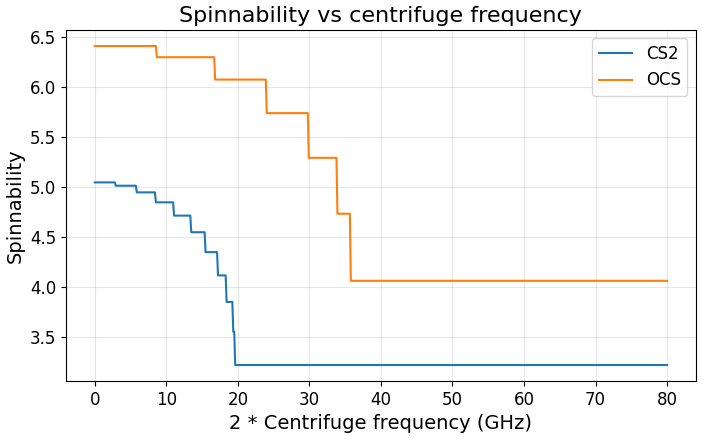
\includegraphics[width=.7\linewidth]{pic/modeling_spinnability.png}
  \end{minipage}\hfill
  \begin{minipage}[c]{0.30\textwidth}
    \small
    \begin{itemize}
      \item does not really explain the different behaviors of the molecules
      \item model assumes \textbf{field-free} states
    \end{itemize}
\end{minipage}
\end{frame}

\subsection{In-Field Rotation}
\begin{frame}{Hamiltonian for Field-Dressed States}

\small
The rotating-frame Hamiltonian

\begin{equation}
\hat H_{\mathrm{dressed}}(t)
=
B \hat J^2
-
D \hat J^4
-
U_0(t)\cos^2\!\theta
-
\Omega(t)\hat J_z .
\end{equation}

\vspace{0.5em}

\textbf{Interpretation:}
\begin{itemize}
    \item \(B\hat J^2 - D\hat J^4\): field-free rotational structure
    \item \(-U_0(t)\cos^2\theta\): aligning interaction with the laser field
    \item \(-\Omega(t)\hat J_z\): rotation-frame term favoring co-rotating angular momentum
    \item The instantaneous eigenstates of \(\hat H_{\mathrm{dressed}}(t)\) are the \textbf{field-dressed states}
    \item In the adiabatic limit, the molecule follows one of these dressed states as \(U_0(t)\) and \(\Omega(t)\) evolve
\end{itemize}


\end{frame}

\begin{frame}{Field Dressed States}
    \centering
    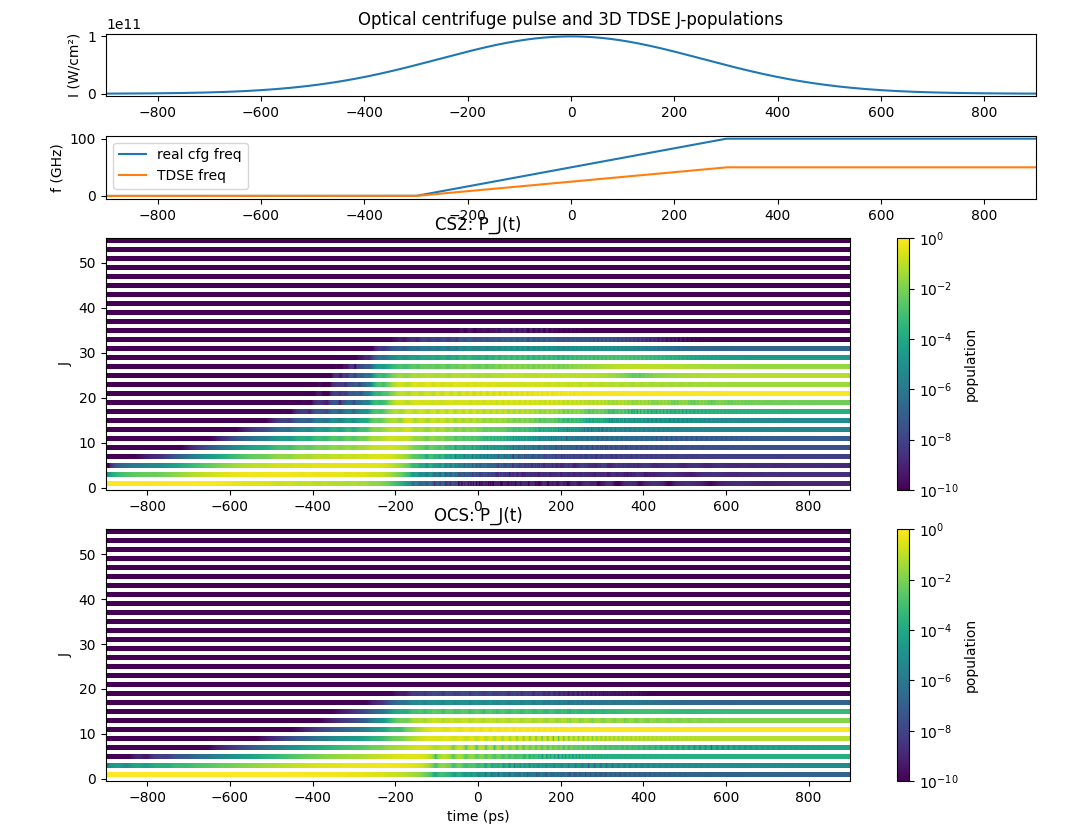
\includegraphics[width=.65\linewidth]{pic/in_field_states.png}
\end{frame}